% This LaTeX document needs to be compiled with XeLaTeX.
\documentclass[10pt]{article}
\usepackage[utf8]{inputenc}
\usepackage{amsmath}
\usepackage{amsfonts}
\usepackage{amssymb}
\usepackage[version=4]{mhchem}
\usepackage{stmaryrd}
\usepackage{graphicx}
\usepackage[export]{adjustbox}
\graphicspath{ {./images/} }
\usepackage{multirow}
\usepackage[fallback]{xeCJK}
\usepackage{polyglossia}
\usepackage{fontspec}
\setCJKmainfont{Noto Serif CJK TC}

\setmainlanguage{polish}
\setmainfont{CMU Serif}

\title{\(\square\) MATEMATYKA -poziom rozszerzony }

\author{}
\date{}


\begin{document}
\maketitle
\(\qquad\)\\
\(\qquad\)

MAJ 2019 LSCDN

\section*{Instrukcja dla zdającego}
\begin{enumerate}
  \item Sprawdź, czy arkusz zawiera 16 stron (zadania 1-16). Ewentualny brak zgłoś przewodniczącemu zespołu nadzorującego egzamin.
  \item Rozwiązania zadań i odpowiedzi zamieść w miejscu na to przeznaczonym.
  \item Odpowiedzi do zadań zamkniętych (1-5) przenieś na kartę odpowiedzi, zaznaczając je w części karty przeznaczonej dla zdającego. Zamaluj pola do tego przeznaczone. Błędne zaznaczenie otocz kółkiem i zaznacz właściwe.
  \item Pamiętaj, że pominięcie argumentacji lub istotnych obliczeń w rozwiązaniu zadania otwartego (7-16) może spowodować, że za to rozwiązanie nie otrzymasz pełnej liczby punktów.
  \item Pisz czytelnie i używaj tylko długopisu lub pióra z czarnym tuszem lub atramentem.
  \item Nie używaj korektora, a błędne zapisy wyraźnie przekreśl.
  \item Pamiętaj, że zapisy w brudnopisie nie będą oceniane.
  \item Możesz korzystać z zestawu wzorów matematycznych, cyrkla i linijki oraz kalkulatora prostego.
  \item Na tej stronie oraz na karcie odpowiedzi wpisz swój kod (nazwisko i imię - zgodnie z ustaleniami szkolnymi).
  \item Nie wpisuj żadnych znaków w części przeznaczonej dla egzaminatora.
\end{enumerate}

Życzymy powodzenia!\\
Liczba punktów\\
do uzyskania: 50

W zadaniach o numerach od 1 do 5 wybierz i zaznacz na karcie odpowiedzi jedną poprawną odpowiedź

\section*{Zadanie 1. (1pkt)}
Liczba \(\sqrt{(1-\sqrt{2})^{2}}+\sqrt{(2-\sqrt{2})^{2}}\) jest równa:\\
A. 1\\
B. \(3+2 \sqrt{2}\)\\
C. 1\\
D. \(2 \sqrt{2}-1\)

Zadanie 2. (1pkt)\\
Wartość wyrażenia \(1-|3 x+|2 x-4||\), dla \(x=-\sqrt{5}\) jest równa:\\
A. \(\sqrt{5}-3\)\\
B. \(2 \sqrt{5}+3\)\\
C. \(3+\sqrt{5}\)\\
D. \(-\sqrt{5}+3\)

Zadanie 3. (1pkt)\\
Liczba \(x=\log _{2} 7+\log _{4} 25+\log _{8} 125\) jest równa\\
A. \(\log _{2} 175\)\\
B. \(\log _{4} 175\)\\
C. \(\log _{2} 150\)\\
D. \(\log _{4} 150\)

Zadanie 4. (1pkt)\\
Liczba 0,3 jest jednym z przybliżeń liczby \(\frac{5}{16}\). Błąd względny tego przybliżenia, wyrażony w procentach, jest równy\\
A. \(4 \%\)\\
B. \(0,04 \%\)\\
C. \(2,5 \%\)\\
D. \(0,025 \%\)

\section*{Zadanie 5. (1pkt)}
Dane są trzy okręgi o środkach A, B, C i promieniach równych odpowiednio r, 2r, 3r. Każde dwa z tych okręgów są zewnętrznie styczne. Jeżeli \(\angle A C B=\alpha\) zaś \(\angle A B C=\beta\) wówczas\\
A. \(\sin \beta=\frac{3}{5}\)\\
B. \(\sin \alpha=\frac{3}{5}\)\\
C. \(\operatorname{tg} \alpha=\frac{4}{3}\)\\
D. \(\operatorname{tg} \beta=\frac{3}{4}\)\\

\includegraphics[max width=\textwidth, center]{2024_11_21_439e1d90cd1e7f928ae2g-03}

\section*{Zadanie 6. (2pkt)}
Wyznacz liczbę \(x=\left(3-\frac{\sqrt{3}}{2}\right)^{3}\). Zakoduj cyfrę jedności i dwie początkowe cyfry po przecinku rozwinięcia dziesiętnego otrzymanego wyniku.

\begin{center}
\begin{tabular}{|l|l|l|}
\hline
\multirow{2}{*}{jedności} & \multicolumn{2}{|c|}{części} \\
\cline { 2 - 3 }
 & dziesiętne setne &  \\
\hline
\end{tabular}
\end{center}

\begin{center}

\includegraphics[max width=\textwidth]{2024_11_21_439e1d90cd1e7f928ae2g-04}
\end{center}

Rozwiązania zadań od 7 do 15 należy zapisać w wyznaczonych miejscach pod treścią zadania.

\section*{Zadanie 7. (4pkt)}
Rozwiąż równanie \(3|x+2|=|x-3|+11\)\\

\includegraphics[max width=\textwidth, center]{2024_11_21_439e1d90cd1e7f928ae2g-05}

\section*{Zadanie \(8 . \quad(4 \mathrm{pkt})\).}
Uzasadnij, że jeśli \(b \neq c, a \neq b, a \neq c\) i \(a+b=2 c\) to \(\frac{a}{a-c}+\frac{b}{b-c}=2\)\\

\includegraphics[max width=\textwidth, center]{2024_11_21_439e1d90cd1e7f928ae2g-06}

Zadanie 9. (5pkt).\\
Wiedząc, że \(\sin \alpha+\cos \alpha=\frac{1}{\sqrt{2}}\). Oblicz wartość wyrażenia \(\sin ^{3} \alpha+\cos ^{3} \alpha\).\\

\includegraphics[max width=\textwidth, center]{2024_11_21_439e1d90cd1e7f928ae2g-07}

Zadanie 10. (4pkt)\\
Wyznacz wszystkie wartości parametru a, gdzie a należy do zbioru liczb całkowitych i \(a \neq 0\), dla których liczba \(x=\frac{4 a-15}{a}\) jest liczbą naturalną.\\

\includegraphics[max width=\textwidth, center]{2024_11_21_439e1d90cd1e7f928ae2g-08}

Zadanie 11. (4pkt)\\
W trójkącie ostrokątnym ABC wysokości AD i BE przecinają się w punkcie S .\\
Wiadomo, że \(|A D|+|B E|=20, \quad|A S|=8, \quad|B S|=4\).\\
Wyznacz długości odcinków DS i ES.\\

\includegraphics[max width=\textwidth, center]{2024_11_21_439e1d90cd1e7f928ae2g-09}

\section*{Zadanie 12. ( 3pkt}
Dla jakich cyfr x i y \((x \neq y)\) liczba 35x24y jest podzielna przez 45?\\
( y - jest to cyfra jedności, a x - cyfra tysięcy)\\
Odpowiedź uzasadnij.

Zadanie 13. (4pkt)\\
Dany jest prostokąt \(A B C D\), w którym \(|A B|=10,|B C|=6\). Odcinek AE jest wysokością trójkąta DAB opuszczoną na jego bok BD. Oblicz pole trójkąta AED.\\

\includegraphics[max width=\textwidth, center]{2024_11_21_439e1d90cd1e7f928ae2g-11}

Zadanie 14. (5pkt)\\
Uczniowie klasy 3a napisali prace klasową z matematyki. Oceny bardzo dobre otrzymało 30\% uczniów, oceny dobre \(40 \%\) uczniów, oceny dostateczne 8 uczniów, a pozostali uczniowie otrzymali oceny dopuszczające. Średnia ocen z tej klasówki wynosiła 3,9. Ilu uczniów otrzymało poszczególne oceny?\\

\includegraphics[max width=\textwidth, center]{2024_11_21_439e1d90cd1e7f928ae2g-12}

Zadanie 15. (5pkt)\\
Dany jest trójkąt równoboczny o boku długości 16. Na boku BC obrano punkt P dzielący ten bok w stosunku 3 : 5, licząc od punktu B. Oblicz sinus kąta BAP.\\

\includegraphics[max width=\textwidth, center]{2024_11_21_439e1d90cd1e7f928ae2g-13}

\section*{Zadanie 16. (5pkt)}
Wspólne styczne dwóch okręgów stycznych zewnętrznie przecinają się pod kątem \(60^{\circ}\). Wyznacz stosunek promieni tych okręgów.\\

\includegraphics[max width=\textwidth, center]{2024_11_21_439e1d90cd1e7f928ae2g-14}

\begin{center}
\begin{tabular}{|c|c|c|c|c|c|c|c|c|c|c|c|c|c|c|c|c|c|c|c|c|c|c|c|}
\hline
到 &  &  &  &  &  &  &  &  &  &  &  &  &  &  &  &  &  &  &  &  &  &  &  \\
\hline
, &  &  &  &  &  &  &  &  &  &  &  &  &  &  &  &  &  &  &  &  &  &  &  \\
\hline
 &  &  &  &  &  &  &  &  &  &  &  &  &  &  &  &  &  &  &  &  &  &  &  \\
\hline
- &  &  &  &  &  &  &  &  &  &  &  &  &  &  &  &  &  &  &  &  &  &  &  \\
\hline
- &  &  &  &  &  &  &  &  &  &  &  &  &  &  &  &  &  &  &  &  &  &  &  \\
\hline
- &  &  &  &  &  &  &  &  &  &  &  &  &  &  &  &  &  &  &  &  &  &  &  \\
\hline
- &  &  &  &  &  &  &  &  &  &  &  &  &  &  &  &  &  &  &  &  &  &  &  \\
\hline
- &  &  &  &  &  &  &  &  &  &  &  &  &  &  &  &  &  &  &  &  &  &  &  \\
\hline
- &  &  &  &  &  &  &  &  &  &  &  &  &  &  &  &  &  &  &  &  &  &  &  \\
\hline
 &  &  &  &  &  &  &  &  &  &  &  &  &  &  &  &  &  &  &  &  &  &  &  \\
\hline
- &  &  &  &  &  &  &  &  &  &  &  &  &  &  &  &  &  &  &  &  &  &  &  \\
\hline
 &  &  &  &  &  &  &  &  &  &  &  &  &  &  &  &  &  &  &  &  &  &  &  \\
\hline
 &  &  &  &  &  &  &  &  &  &  &  &  &  &  &  &  &  &  &  &  &  &  &  \\
\hline
 &  &  &  &  &  &  &  &  &  &  &  &  &  &  &  &  &  &  &  &  &  &  &  \\
\hline
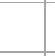
\includegraphics[max width=\textwidth]{2024_11_21_439e1d90cd1e7f928ae2g-15(1)}
 &  &  &  &  &  &  &  &  &  &  &  &  &  &  &  &  &  &  &  &  &  &  &  \\
\hline
 &  &  &  &  &  &  &  &  &  &  &  &  &  &  &  &  &  &  &  &  &  &  &  \\
\hline
 &  &  &  &  &  &  &  &  &  &  &  &  &  &  &  &  &  &  &  &  &  &  &  \\
\hline
 &  &  &  &  &  &  &  &  &  &  &  &  &  &  &  &  &  &  &  &  &  &  &  \\
\hline
 &  &  &  &  &  &  &  &  &  &  &  &  &  &  &  &  &  &  &  &  &  &  &  \\
\hline
 &  &  &  &  &  &  &  &  &  &  &  &  &  &  &  &  &  &  &  &  &  &  &  \\
\hline
 &  &  &  &  &  &  &  &  &  &  &  &  &  &  &  &  &  &  &  &  &  &  &  \\
\hline
- &  &  &  &  &  &  &  &  &  &  &  &  &  &  &  &  &  &  &  &  &  &  &  \\
\hline
 &  &  &  &  &  &  &  &  &  &  &  &  &  &  &  &  &  &  &  &  &  &  &  \\
\hline

\includegraphics[max width=\textwidth]{2024_11_21_439e1d90cd1e7f928ae2g-15}
 &  &  &  &  &  &  &  &  &  &  &  &  &  &  &  &  &  &  &  &  &  &  &  \\
\hline
- &  &  &  &  &  &  &  &  &  &  &  &  &  &  &  &  &  &  &  &  &  &  &  \\
\hline
 &  &  &  &  &  &  &  &  &  &  &  &  &  &  &  &  &  &  &  &  &  &  &  \\
\hline
- &  &  &  &  &  &  &  &  &  &  &  &  &  &  &  &  &  &  &  &  &  &  &  \\
\hline
 &  &  &  &  &  &  &  &  &  &  &  &  &  &  &  &  &  &  &  &  &  &  &  \\
\hline
 &  &  &  &  &  &  &  &  &  &  &  &  &  &  &  &  &  &  &  &  &  &  &  \\
\hline
 &  &  &  &  &  &  &  &  &  &  &  &  &  &  &  &  &  &  &  &  &  &  &  \\
\hline
 &  &  &  &  &  &  &  &  &  &  &  &  &  &  &  &  &  &  &  &  &  &  &  \\
\hline
 &  &  &  &  &  &  &  &  &  &  &  &  &  &  &  &  &  &  &  &  &  &  &  \\
\hline
 &  &  &  &  &  &  &  &  &  &  &  &  &  &  &  &  &  &  &  &  &  &  &  \\
\hline
 &  &  &  &  &  &  &  &  &  &  &  &  &  &  &  &  &  &  &  &  &  &  &  \\
\hline
 &  &  &  &  &  &  &  &  &  &  &  &  &  &  &  &  &  &  &  &  &  &  &  \\
\hline
 &  &  &  &  &  &  &  &  &  &  &  &  &  &  &  &  &  &  &  &  &  &  &  \\
\hline
 &  &  &  &  &  &  &  &  &  &  &  &  &  &  &  &  &  &  &  &  &  &  &  \\
\hline
 &  &  &  &  &  &  &  &  &  &  &  &  &  &  &  &  &  &  &  &  &  &  &  \\
\hline
 &  &  &  &  &  &  &  &  &  &  &  &  &  &  &  &  &  &  &  &  &  &  &  \\
\hline
 &  &  &  &  &  &  &  &  &  &  &  &  &  &  &  &  &  &  &  &  &  &  &  \\
\hline
 &  &  &  &  &  &  &  &  &  &  &  &  &  &  &  &  &  &  &  &  &  &  &  \\
\hline
 &  &  &  &  &  &  &  &  &  &  &  &  &  &  &  &  &  &  &  &  &  &  &  \\
\hline
 &  &  &  &  &  &  &  &  &  &  &  &  &  &  &  &  &  &  &  &  &  &  &  \\
\hline
 &  &  &  &  &  &  &  &  &  &  &  &  &  &  &  &  &  &  &  &  &  &  &  \\
\hline
\end{tabular}
\end{center}

WYPELNIA PISZĄCY

\begin{center}
\begin{tabular}{|l|c|c|c|c|}
\hline
\begin{tabular}{c}
\(\mathbf{N r}\) \\
zadania \\
\end{tabular} & A & B & C & D \\
\hline
1. & \(\square\) & \(\square\) & \(\square\) & \(\square\) \\
\hline
2. & \(\square\) & \(\square\) & \(\square\) & \(\square\) \\
\hline
3. & \(\square\) & \(\square\) & \(\square\) & \(\square\) \\
\hline
4. & \(\square\) & \(\square\) & \(\square\) & \(\square\) \\
\hline
\(\mathbf{5 .}\) & \(\square\) & \(\square\) & \(\square\) & \(\square\) \\
\hline
\end{tabular}
\end{center}

WYPEENIA SPRAWDZAJACY

\begin{center}
\begin{tabular}{|l|c|c|}
\hline
\begin{tabular}{c}
Nr \\
zadania \\
\end{tabular} & \(\mathbf{0}\) & \(\mathbf{2}\) \\
\hline
\(\mathbf{6 .}\) & \(\square\) & \(\square\) \\
\hline
\end{tabular}
\end{center}

\begin{center}
\begin{tabular}{|l|c|c|c|c|c|c|}
\hline
\begin{tabular}{c}
Nr \\
zadania \\
\end{tabular} & \(\mathbf{0}\) & \(\mathbf{1}\) & \(\mathbf{2}\) & \(\mathbf{3}\) & \(\mathbf{4}\) & \(\mathbf{5}\) \\
\hline
\(\mathbf{7 .}\) & \(\square\) & \(\square\) & \(\square\) & \(\square\) & \(\square\) &  \\
\hline
\(\mathbf{8 .}\) & \(\square\) & \(\square\) & \(\square\) & \(\square\) & \(\square\) &  \\
\hline
\(\mathbf{9 .}\) & \(\square\) & \(\square\) & \(\square\) & \(\square\) & \(\square\) & \(\square\) \\
\hline
\(\mathbf{1 0 .}\) & \(\square\) & \(\square\) & \(\square\) & \(\square\) & \(\square\) &  \\
\hline
\(\mathbf{1 1 .}\) & \(\square\) & \(\square\) & \(\square\) & \(\square\) & \(\square\) &  \\
\hline
\(\mathbf{1 2 .}\) & \(\square\) & \(\square\) & \(\square\) & \(\square\) &  &  \\
\hline
\(\mathbf{1 3 .}\) & \(\square\) & \(\square\) & \(\square\) & \(\square\) & \(\square\) &  \\
\hline
\(\mathbf{1 4 .}\) & \(\square\) & \(\square\) & \(\square\) & \(\square\) & \(\square\) & \(\square\) \\
\hline
\(\mathbf{1 5 .}\) & \(\square\) & \(\square\) & \(\square\) & \(\square\) & \(\square\) & \(\square\) \\
\hline
\(\mathbf{1 6 .}\) & \(\square\) & \(\square\) & \(\square\) & \(\square\) & \(\square\) & \(\square\) \\
\hline
\end{tabular}
\end{center}

\begin{center}
\begin{tabular}{|c|c|}
\hline
\begin{tabular}{c}
Suma punktów \\
zadania otwarte \\
\end{tabular} &  \\
\hline
 &  \\
\hline
\end{tabular}
\end{center}


\end{document}